\chapter{IDEA testbeams}

\epigraph{New quote split \\ over two lines}{Author McWriter}

While DQM4hep was intended as a generic tool, it was largely developed within the AIDA-2020 collaboration, which also promoted a variety of standardisations for data acquisition devices, data formats, etc. In order to test whether DQM4hep was truly generic, and able to adapt to any type of detector, it needed to be tested outside of the AIDA-2020 groups and facilities. An ideal opportunity was presented for this, with a collaboration of Italian universities working on a number of particle detectors, hoping to do a single combined testbeam at the CERN SPS. 

[...]

\section{Introduction}
The combined testbeam took place between 5th-12th September 2018 at the CERN SPS beamline facility. [...]

\subsection{Detectors present at the combined testbeam}
The combined testbeam comprised four separate dectors: a calorimeter, a muon detector and preshower, a drift chamber, and a silicon photomultiplier. One of the biggest challenges involved in the testbeam was operating these four different detectors [...]

\subsubsection{RD52 calorimeter}
The calorimeter was formed of two layers of 36 tiles each, totaling 72 tiles, stacked behind each other. One layer used Cherenkov detectors, the other used scintillator tiles. In addition, there was a group of leakage detectors that detected whether individual events were contained within the calorimeter or not. [DWC - Delayed Wire Chamber?]

\subsubsection{Muon chamber and preshower}
[...]

\subsubsection{Silicon photomultiplier GEM}
[...]

\subsubsection{Drift chamber}
[...]

\section{Progression of the testbeam} % Little awkward title
[...]

Existing monitoring within the DREAM collaboration could produce accurate histograms from raw data using ROOT, creating plots of the energy spectra of each detector channel per event, along with [other things]. This facility was reproduced in DQM4hep quickly using for-loops in both the C++ code and XML steering files, allowing this to be done with comparatively little code.

\subsection{File readers}
[...]

The RD52 calorimeter, drift chamber, and muon and preshower were all read using ROOT ntuple files, generated by the DAQ one step after reading and saving the data in a raw binary format. This made the file reader code simpler, faster and more readable, as it only needed to walk through ROOT trees and extract data from leaves event-by-event, rather than reading from raw binary or hex data.

For the silicon photomultiplier GEM data, the ``raw'' data format was a text file, containing an XML header followed by a large amount of data in comma-separated values (CSV). This file could be loaded directly into DQM4hep, the XML header separated and parsed with DQM4hep's internal XML parsing libraries, and the remaining data parsed. The comma-separated values could be easily parsed using the \texttt{dqm4hep::core::tokenize} function, which takes a string, a delimiter, and a vector, and parses the string into values separated by the delimiter, loading them into the vector. This made extracting the GEM data extremely simple, even in this format.

\subsection{Analysis modules}
[...]

\section{Results}
[...]

\subsection{ADC to energy calibration}
[...]

This required several runs whose characteristics were similar or identical, except for the energy of the beam. The runs chosen where run numbers [...], summarised in Table [ref].

A plot was made of the average ADC per event summed over all channels, against the beam energy for that run. See Fig. [ref]. Then using a linear least squares fit, the equation that describes the transformation from ADC to energy was found.

[...]

\subsection{Tower ADC calibration}
[...]

Due to a large number of tasks for setting up the testbeam, there was not time to perform a high voltage calibration on the individual towers of the calorimeter, so the calorimeter ADCs were not calibrated to each other [?]. In order to fix this, 

For this purpose, a dedicated set of calibration runs were taken. There were 29 calibration runs, all using a 20 GeV electron beam, each pointed at towers 1-29. Towers 30-36 did not receive these calibration runs because [reason]. The run numbers corresponding to each tower is given in Table \ref{table:idea/calibrationruns}.

\begin{table}[h]
\centering
	\begin{tabular}{ c c | c c }
	\hline \hline
	\textbf{Tower} & \textbf{Run No.} & \textbf{Tower} & \textbf{Run No.} \\ \hline \hline
	 1 & 12545 & 16 & 12526 \\
	 2 & 12556 & 17 & 12567 \\
	 3 & 12558 & 18 & 12633 \\
	 4 & 12560 & 19 & 12591 \\
	 5 & 12601 & 20 & 12612 \\
	 6 & 12638 & 21 & 12530 \\
	 7 & 12598 & 22 & 12528 \\
	 8 & 12514 & 23 & 12569 \\
	 9 & 12518 & 24 & 12639 \\
	10 & 12521 & 25 & 12610 \\
	11 & 12600 & 26 & 12609 \\
	12 & 12636 & 27 & 12607 \\
	13 & 12539 & 28 & 12604 \\
	14 & 12628 & 29 & 12602 \\
	15 & 12512 &    &    \\ \hline
	\end{tabular}
	\caption{Table of the run numbers and corresponding tower numbers for the calibration runs.}
	\label{table:idea/calibrationruns}
\end{table}

The process for calibrating the towers was to [...] This created a plot of the distribution of raw ADCs in all towers, shown in Fig. \ref{figure:testbeam/results/calibrationbefore}. Creating a plot of all the data in all of the calibration runs, the mean value on the y-axis was 180.8 GeV for the scintillator, and 178.4 GeV for the Cherenkov. These values were chosen as the average to calibrate to, then a series of calibration coefficients applied to the other channels. These calibration coefficients are shown on Table \ref{table:idea/calibrationcoeffs}.

\begin{table}[h]
\centering
	\begin{tabular}{ c c | c c }
	\hline \hline
	\textbf{Tower} & \textbf{Coefficient} & \textbf{Tower} & \textbf{Coefficient} \\ \hline \hline
	 1 & x & 16 & x \\
	 2 & x & 17 & x \\
	 3 & x & 18 & x \\
	 4 & x & 19 & x \\
	 5 & x & 20 & x \\
	 6 & x & 21 & x \\
	 7 & x & 22 & x \\
	 8 & x & 23 & x \\
	 9 & x & 24 & x \\
	10 & x & 25 & x \\
	11 & x & 26 & x \\
	12 & x & 27 & x \\
	13 & x & 28 & x \\
	14 & x & 29 & x \\
	15 & x &    &    \\ \hline
	\end{tabular}
	\caption{Table of tower numbers and their calibration coefficients.}
	\label{table:idea/calibrationcoeffs}
\end{table}

\begin{figure}[h]
	\centering
	
\includegraphics[width=0.65\textwidth]{../Pictures/Placeholder.png}
	\caption{The plot of ADCs for each tower before calibration.}
	\label{figure:testbeam/results/calibrationbefore}
\end{figure}

\begin{figure}[h]
	\centering
	
\includegraphics[width=0.65\textwidth]{../Pictures/Placeholder.png}
	\caption{Comparison of the calibration plots for the ADCs before and after calibration.}
	\label{figure:testbeam/results/calibrationafter}
\end{figure}

\subsection{Particle selection efficiencies}
[...]

\subsubsection{Using the ancillary detectors}
[...]

\subsubsection{Using the calorimeter}
[...]

One of the first steps is using the RD52 calorimeter data to find the energy ratio $R$ for each event:

\begin{displaymath}
	R = \frac{E_1}{\sum_{i=1}^{n} E_i}
\end{displaymath}

where $E_i$ is the energy of the $i^{th}$ most energetic channel in the event and $n$ is a nonzero integer. The choice of $n$ [...]. Once the ratio $R$ is calculated, a plot can be made of $E_{total}$ vs. $R$ for an entire run that shows separation of electrons from muons and pions -- see Fig. \ref{figure:testbeam/results/EvR}.

% Replace this diagram with the updated one (though probably *after* we've normalised for beam energy).
% Also, Run 12709 is an electron run, not a hadron run!

\begin{figure}[h]
	\centering
	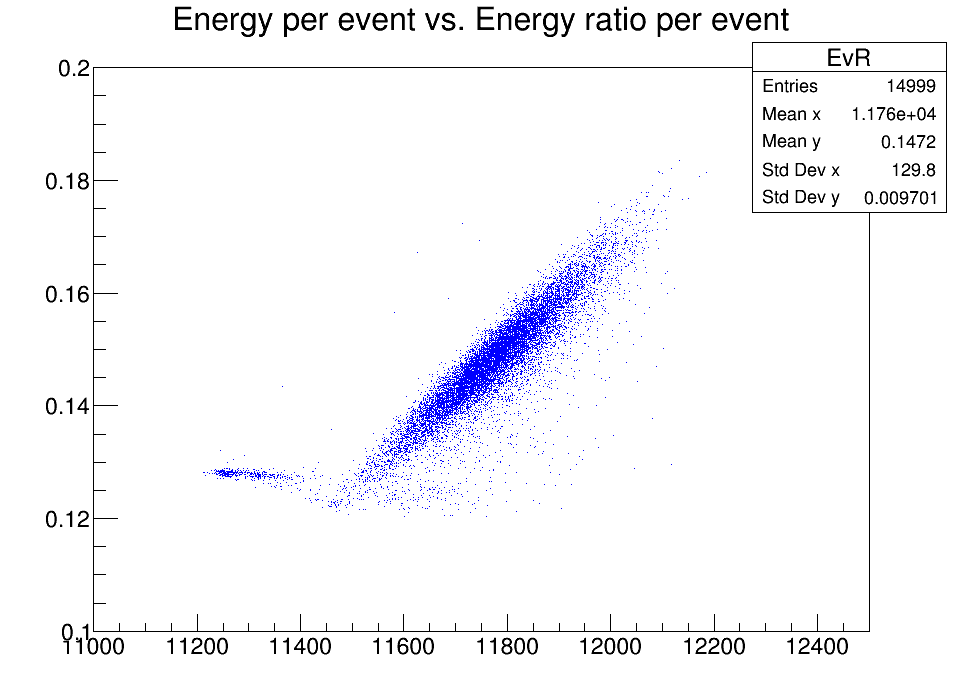
\includegraphics[width=0.65\textwidth]{../Pictures/12709-EvR.png}
	\caption{Plot of $E$ against $R$ for the secondary hadron beam with $n = 10$ (Run 12709).}
	\label{figure:testbeam/results/EvR}
\end{figure}

An appropriate cut can be used to select electron events. [Information about the cut]. Adding in the information from the RD52's muon trigger, muons and pions can then also be separated. Using both the cut and the muon trigger, we can thus produce spectra for each individual type of particle in the run.

[...]

The main goal of the data analysis is to characterise the response of the detector, and to measure the selection efficiencies of the detectors to various particle types. Once this is done, this will also give us a detailed account of the beam composition during each of the runs, which can be used for further work.

In order to do this, several ways to select for different particle types are necessary. The first way was using the preshower detector and muon trigger, which are both designed to discriminate between electrons and muons (respectively), with a high selection efficiency. These are used to create ``reference'' samples, [...]

The second way is to perform a kinematic selection using variables from the calorimeter. This is done using the E vs. R plot (normalised for beam energy) to select a region corresponding to a certain particle type. For example, the plot below shows this plot for Run [xxx] (X GeV hadrons) with the regions corresponding to hadrons and electrons highlighted. These regions overlap, meaning that attempting to select for hadrons using an ellipse around that region will also result in a non-insignificant number of electrons also being selected.

In order to perform a pure selection using the calorimeter, an extremely tight cut was used, focusing on the red spot at the centre of the hadron region. This ensures that the majority of events that pass the cut are hadrons, giving a high-purity selection. The purity of this selection can be assessed by using the appropriate preshower or muon trigger, excluding all non-hadron particles, and comparing the two numbers. If $N_{K}$ is the number of particles passing the selection with only the kinematic cut, and $N_{K+T}$ is the number of particles passing \emph{both} the kinematic cut and the triggers, then the selection efficiency for hadrons $\epsilon_{hadron}$ is given by:

\begin{displaymath}
	\epsilon_{hadron} = \frac{N_{K+T}}{N_{K}}
\end{displaymath}

This was then done with the same process for electrons and muons, to obtain the individual selection efficiencies. % Should probably go through the process with the actual cut values itself.

% Results of this selection, and the matrix?